\documentclass[runningheads]{llncs}
\usepackage[utf8]{inputenc}
%\usepackage[top=1in, bottom=1in, left=1in, right=1in]{geometry}
% \usepackage{times}
\usepackage{amsmath}

%\usepackage{amsmath}
\usepackage{graphicx}
%\usepackage{setspace}
%\usepackage{subfig}
%\usepackage[hyphens]{url}
\usepackage{hyperref}
\usepackage{xspace}
\usepackage{color}
%\usepackage{flushend}
\usepackage{paralist}
\usepackage[ruled,vlined]{algorithm2e}
\usepackage{enumitem}

\usepackage{caption}
\usepackage{tabularx}
\usepackage[]{todonotes}

  
\newcommand{\sys}{Promise\xspace}
\newcommand{\discount}{\sum_{t=0}^{T} \big( \frac{\delta}{1+r} \big)^t}

\newcommand{\todoin}[1]{\todo[inline,caption={}]{#1}}
\newcommand{\toall}[1]{\todo[linecolor=orange,backgroundcolor=orange!25,bordercolor=orange,inline, caption={}]{Unassigned Todo: #1}}

\newcommand{\aza}[1]{\todo[linecolor=blue,backgroundcolor=blue!25,bordercolor=blue,inline,caption={}]{Comment by Alexei: #1}}
\newcommand{\toaza}[1]{\todo[linecolor=blue,backgroundcolor=blue!25,bordercolor=blue,inline,caption={}]{Todo for Alexei: #1}}

\newcommand{\rk}[1]{\todo[linecolor=red,backgroundcolor=red!25,bordercolor=blue,inline,caption={}]{Comment by Rami: #1}}
\newcommand{\tork}[1]{\todo[linecolor=blue,backgroundcolor=red!25,bordercolor=red,inline,caption={}]{Todo for Rami: #1}}

\newcommand{\lgu}[1]{\todo[linecolor=yellow,backgroundcolor=yellow!25,bordercolor=yellow,inline,caption={}]{Comment by Lewis: #1}}
\newcommand{\tolgu}[1]{\todo[linecolor=yellow,backgroundcolor=yellow!25,bordercolor=yellow,inline,caption={}]{Todo for Lewis: #1}}

\newcommand{\dom}[1]{\todo[linecolor=green,backgroundcolor=green!25,bordercolor=green,inline,caption={}]{Comment by Dominik: #1}}
\newcommand{\todom}[1]{\todo[linecolor=green,backgroundcolor=green!25,bordercolor=green,inline,caption={}]{Todo for Dominik: #1}}

\begin{document}

\title{
\sys: Leveraging Future Gains for Collateral Reduction in Competitive Markets
% \sys: Leveraging Future Payments for Bootstrapping Collateralized Protocols
} 
\author{
\institute{}
}


\date{}
\maketitle

%-------------------------------------------------
%---------------ABSTRACT------------------------
%-------------------------------------------------

\begin{abstract}
\dom{Proposal: change the paper to restrict the mechanism to protocols in which there is competition, i.e. Bob can exit when Alice is malicious. I think one of the biggest problems is that \sys does not work when you have a monopoly situation.}
Collateral employed in cryptoeconomic protocols protects against the misbehaviour of economically rational agents, compensating honest users for damages and punishing misbehaving parties.
%It can increase the trustworthiness of a system by compensating honest users for damages and revoking the locked capital of cheating parties.
The introduction of collateral, however, carries two disadvantages: (i) requiring actors to lock up substantial amount of collateral can be an entry barrier, limiting the set of candidates to wealthy agents; and (ii) affected agents incur ongoing opportunity costs as the collateral cannot be utilized elsewhere.
%First, a substantial lockup requirement can act as a barrier to entry for certain protocol roles, limiting the set of candidates to wealthy agents.
%Second, agents incur ongoing opportunity costs while their collateral is locked up, as it cannot be utilized elsewhere.

We present \sys, a mechanism to decrease the initial capital requirements of economically rational service providers in cryptoeconomic protocols.
\sys leverages future income (e.g. transaction fees) prepaid by users to reduce the collateral actively locked up by service providers, while sustaining secure operation of the protocol.
We provide a model for evaluating the effectiveness of \sys and argue its security.
% Lastly, we discuss how \sys can be applied to existing second-layer scaling, blockchain interoperability, and decentralized mining protocols.
%allowing the required collateral to be constituted by future transaction fees by the user, while \emph{sustaining the overall collateral} required as a security deposit.
%Using \sys, a user can force a service provider to lock payments as future collateral.
%Further, the user is able to provide multiple future payments in escrow to provide a revenue guarantee to a service provider.
%We show that, using \sys, delayed payments securely held in escrow can be fairly distributed after the predefined delay.
%We further argue that \sys motivates users to lock future payments as collateral and intermediaries have higher overall collateral.
% We further show that \sys leads to a Nash equilibrium where some agent roles are motivated to lock future payments as collateral to motivate other agent roles to behave honestly without degrading the overall security provided by a system.
%\dom{Do we need that layer-two mention in there? I think Promise as a scheme is also applicable to layer 1?}
%\rk{I removed the extra layer-two word. Does interop and decentralized mining count as pure L1?}
%\dom{I was wondering about mining pools (the non-decentralized ones). But I'm not sure. I also think in Bitcoin mining you delay the payout of the reward a couple of blocks by default because of the lack of finality. What do you think?}
%\rk{It's not exactly the same, because you can initiate a transfer from the miner's wallet to a recipient immediately in the next block, right? You can play "hot potato" with the mining reward.}
%Lastly, we elaborate on applying \sys to several commonly known protocols, including second-layer scaling, blockchain interoperability, and decentralized mining protocols.
%\rk{If we don't provide full example texts for things other than nocust then: Lastly, we elaborate on applying \sys to second-layer scaling.
%}
\end{abstract}

%-------------------------------------------------
%---------------INTRODUCTION------------------------
%-------------------------------------------------

\section{Introduction}
\label{sec:intro}

% \dom{TODO:
% \begin{itemize}
%     \item The intro should be 3/4 pages max
%     \item Make problem statement concise
%     \item clean up intuition
%     \item make sure assumptions are complete
% \end{itemize}}

Since their creation, arguably the most significant property of blockchains is their facilitation of trustless exchange between entities with \emph{weak identities}~\cite{rainer}~\footnote{Agents with \emph{weak} identities are able to suddenly leave a network; agents with \emph{strong} identities cannot.}.
Yet the trustless nature of the systems means not only that parties \textit{may} transact without trusting each other, but also that they \textit{should not trust} each other.
%\footnote{Or at least should not trust each other.}.
This creates a design challenge for interactions which would typically involve such trust. 
% In this paper, we focus on blockchain protocols which, at least in part, express \textit{trust} through \textit{collateral}.
%Here, collateral is value escrowed by party A to guarantee party B that A will not misbehave given that A's economic gain from cheating is not higher than the collateral value.
In particular, payment protocols can be designed such that B is guaranteed to receive at least the same amount of funds from A that are at risk.
% Here, collateral is value escrowed by party A to guarantee party B that regardless of the behavior of party A, party B cannot lose funds. 
In this paper, we focus on blockchain protocols which, at least in part, encode \textit{trust} by monetary \textit{collateral}.
%\dom{Definition is a bit tricky, would change that it not only relates to funds but basically under rationality assumption, A would not cheat.}
Here, collateral is value escrowed by party A to guarantee party B that regardless of the behavior of party A, party B cannot lose funds. 
%It allows us to create systems that are resistant against economically rational adversaries by imposing the threat of destroying their money and motivating their honest behavior.
Protocols involving collateral include cross-chain communication~\cite{Zamyatin2019XCLAIM}, scalable off-chain payments~\cite{Khalil2019NOCUST}, state channels~\cite{dziembowski2018general}, and watchtowers~\cite{mccorry2018pisa}.
% avarikioti2019brick avarikioti2018towards
%, and (decentralized) mining pools.\dom{need citation for smartpool and p2pool}
% outsourcing of computation and verification games~\cite{teutsch2017scalable}

% Relying on collateral as a means of trust is associated with a different set of challenges. 
\paragraph{Problem.}
Relying on collateral as trust is itself associated with a different set of challenges. 
Collateralization requires the provision of a substantial amount of funds upon protocol initialization, limiting the set of participants to a selected few.
Leaving participation to a small set of agents can lead to phenomenons like ``rich are getting richer'' through wealth compounding~\cite{Fanti2019Compounding}.
% The concept of equitability in Proof-of-Stake (PoS) protocols explores this phenomenon of the  in this context.
% Wealthy agents are able to earn an absolutely larger proportion of the rewards as their likelihood to earn is increased by their amount of collateral.
% In the permissionless setting, protocols with collateral should ideally be egalitarian, i.e. agents are able to earn rewards proportional to their deposits~\cite{Karakostas2019Egalitarianism}.
While it is not possible to grant less wealthy agents proportionally higher rewards due to Sybil identities, we can lower the entry barrier for agents to join a protocol.
Finally, locked funds result in opportunity costs for the agent who could use their collateral for participating in other protocols~\cite{Harz2019Balance}.

% During a bootstrapping phase, the necessary coins for participating in a protocol needs to be distributed ideally to honest agents.
% However, this is detrimental to the diea of decentralization as 
% which may make it challenging for parties to participate in the protocol.
% In addition, the funds are locked up for the duration of the protocol.
% \aza{Citations here and a bit more detail?}
\paragraph{This work.}
We present \sys, a simple but effective mechanism to lower entry barriers for intermediaries in protocols relying on collateral for secure operation.
Instead of locking up a significant amount of funds as collateral, \sys allows intermediaries to stake their future income, ``promised" for correctly providing the service (i.e., fees), instead.
Similar to online orders in e-commerce, users can choose to pay fees upfront (``forward payments") -- for a some pre-agreed service period.
However, instead of transferring these payments directly to the intermediary, users lock pre-paid fees in a escrow smart contact, preventing theft by either party. 
The intermediary needs to provide the service honestly for the entire period set by the user.
The benefit of this scheme is twofold: (i) the intermediary is incentivized to act honestly while enjoying a lower initial collateral, and (ii) the user can reduce his transaction cost and only pays if the service was provided honestly over his defined period. %, authorized by the smart contract, 
%can leverage the pre-paid funds as collateral to maintain secure operation, reducing the liquidity necessary to launch such services; (ii) the user, on the other hand, can be incentivized via a lower fee rate.
As long as the expected future revenue from correct operation exceeds potential gains by the intermediary, users have the option to leave the protocol, and misbehavior can be proved to the smart contract, \sys incentivizes correct behavior.

\paragraph{Application.}
We apply \sys to NOCUST.
NOCUST is a commit-chain protocol that allows to send cryptocurrency payments off-chain facilitated by so-called operators~\cite{Khalil2019NOCUST}.
Operators are service-providing agents that (i) collect fees for operating the off-chain payment network, and (ii) provide a certain amount of collateral to insure finalization of payments.
We show that with an increasing number of operators, the amount of collateral each operator provides can be \emph{lowered}.
Moreover, we show that the implementation of \sys in an Ethereum Solidity smart contract only adds XX cost for the user and XX cost for the operator.

\paragraph{Outline.}
We introduce the system model and assumptions in Section~\ref{sec:model}, followed by a description of \sys in Section~\ref{sec:promise}.
Next, we discuss the security of \sys in Section~\ref{sec:security}. % and highlight how \sys can be applied to existing systems in Section~\ref{sec:application}.
We discuss related work in Section~\ref{sec:related} and conclude in Section~\ref{sec:conclusion}.

%propose that payments made for successfully completing tasks are made in advance and held in escrow for a period of time determined by a user, sharing the burden of the provision of upfront collateral.
%Thereby, a user can start interacting with an intermediary with a small amount of value at risk and gradually increase the values by forcing the intermediary to use the ongoing payments as additional collateral.
%An intermediary can withdraw surplus collateral when the sum of initially locked collateral and accrued payments is above a user defined overall collateral threshold.
%Moreover, we allow cheating by an intermediary to impact the probability of an agent choosing to interact with the intermediary again.
%That way honest economically rational agents have a higher net reward compared to locking up the collateral initially.
% Also, users have the possibility to obtain a service guarantee over a defined period of time.
% \dom{Let's try to find a way that compensates the intermediary for that. Maybe payment can be increased.}

% Moreover, we allow users to lock future payments in escrow to reduce relative payments.
% To ensure liquidity in the system, a user can lock payments, say for the expected number of tasks for a month, and in return receive a discount on the price for providing the task.
% Locked future payments allow users to reduce their costs and gives intermediaries the chance to better predict demand.
% In turn, locked payments motivates intermediaries to keep collateral locked in the protocol.





%-------------------------------------------------
%---------------MODEL------------------------
%-------------------------------------------------


\section{System Model}
\label{sec:model}

In \sys, a user Bob engages an intermediary Alice to fulfill a task valued at $V_B$ on his behalf.
% For a generic service, Alice and Bob agree on a contract that details which task Alice has to provide.
Bob pays Alice $p$ each period $t$ for performing the task. % for fulling the task.
Given the absence of \textit{strong identities}, the total value of the task to Bob ($V_B$) needs to be fully collateralized, via a deposit $D$, such that $D \geq V_B$.
For example, if a particular task involves Alice offering a service and Bob having a \$100 exposure---in the form of counter-party risk---to Alice, Alice will need to post at least \$100 as collateral to \textit{insure} offset the exposure, such that Bob does not stand to lose funds if Alice behaves maliciously. % and tries to steal them.

Formally, we adopt the definitions of agreements in cryptoeconomic protocols from~\cite{Harz2019Balance}.
The service providing agent Alice $A$ and the receiving agent Bob $B$ participate in an agreement encoded by:

\begin{equation}
	\mathcal{A} = \langle \Phi, p, D \rangle
\end{equation}

In such an agreement, Alice needs to fulfil the specification $\Phi$ and provide the collateral $D$ in advance.
When Alice fulfills the specification, the payment $p$ held in escrow is released to Alice.

\subsection{Specifications}
\dom{We need to explain what specifications are and give some examples here.}


\subsection{Roles}

\sys adopts the BAR model of rational agents~\cite{aiyer2005bar} including private preferences of agents as proposed in~\cite{Harz2019Balance}.
We define the following roles.

\begin{itemize}
    \item \textbf{Alice}, the Intermediary: Alice is economically rational and entrusted with executing a task. She provides a deposit $D$ into the escrow before executing the task and receives a payment $p$ upon successful completion.
    \item \textbf{Bob}, the User: Bob represents the user requesting execution of a task by Alice. A user provides payments $\{p_0, ..., p_m\}$ into the escrow. % Bob can provide multiple future payments into the escrow.
    \item \textbf{Escrow}: The escrow is a smart contract responsible for holding deposits by Alice and payments by Bob.
    \item \textbf{Verifier}: The verifier detects malicious behavior of Alice. In practice, this role is fulfilled by a smart contract, a dedicated third party, or the user.
\end{itemize}

%defined in the specification $\phi$

% \dom{Do we need to define blockchain model with finality assumptions, parameter $k$ etc.?}

% \rk{Would it make sense to rename $D_{min}$ to $D$? Minimum sort of implies that it's already minimized while base can refer to a base value Promise optimizes.}
% \dom{I'm happy with that change.}

% The generic service typically implies a requirement that the value of the task is ``insured'' via a deposit $D$.

% {\color{red}
% [Moved assumptions from intro]
\subsection{Assumptions}

The verifier in the system is able to detect any faults by Alice and is able to prove that Alice was at fault.
% Alice provides a deposit to deter her from behaving maliciously and receives a payment for successfully completing the task.
We further assume that the protocol utilizing \sys implements payments and deposits through a ledger that provides the functionalities as describes in, e.g.~\cite{garay2016bitcoin}.
% The payments and deposits are held in custody by an escrow implemented within the decentralized ledger.
Also, there is a one to one mapping between the collateral and a user, i.e.\ the collateral of an intermediary is not split between multiple users.
Last, agents in the system can be identified with their public/private key pair.


% \begin{itemize}
%     \item Alice and Bob interact with each other
%     \item With \sys, Alice needs to provide less collateral
%     \item Alice has the choice between cheating and being honest in a protocol
%     \item In the early stages of a protocol, if a user experiences cheating, the probability that the user will continue to use the protocol are low
%     \item We can use this "exit probability" as a parameter encoded into the protocol
%     \item The higher the exit probability of users, the less collateral a service provider has to pay
%     \item The service provider has to choose between a guaranteed income and cheating
%     \item However, we assume that in the next round a user might not be available any longer if the user experiences cheating
% \end{itemize}

% \begin{itemize}
%     \item add assumption that the protocols using \sys are able to detect any kind of failures
% \end{itemize}

% }


\subsection{Utilities}
% \dom{This part is repetitive to the start of this section. Revise and shorten here.}
% Consider the following generic setup.
% Alice provides a task with a value of $V_B$ to Bob. % involving a total value $V$.
% The task is arbitrary and of value $V$.
% For example, Bob could pay Alice to be an operator in NOCUST to finalize off-chain payment with value $V$~\cite{Khalil2019NOCUST}.
% Another example involves Alice providing Bob with a digital good using the FairSwap protocol where the good as a value $V$~\cite{fair}.
% \rk{"such that $D_{min} \geq V$". Not a general statement for all protocols we consider though.}
% Alice provides a minimum collateral $D$ upfront, such that $D \geq V_B$.
% This is to ensure that in the event that Alice cheat Bob out of providing the service, Bob can recover at least his original value. %, and possibly more if Alice is overcollateralized.
%  the service that Alice offers to Bob has value---and accordingly,
% Moreover, Bob pays $p$ every time the service is performed.
Alice can either behave honestly or cheat, with the following payoffs one period ahead.
$V_A$ denotes the numerical value that Alice attaches to the act of cheating.
$V_B$ denotes the numerical value that Bob attaches to receiving the service.
$c$ denotes the cost of an individual transaction. 
$\mathrm{E}[r]D$ reflects the expected opportunity cost of locking the capital for one period. %, calculated as $(1+\mathrm{E}[r])D-D$.

%  ($H$) ($C$)

\begin{equation}
\label{eq:status-quo_alice}
\Pi_A = 
\begin{cases}
    p - \mathrm{E}[r]D, & \text{if Alice is honest} \\
    V_A - \mathrm{E}[r]D-D, & \text{if Alice cheats} \\
\end{cases}
\end{equation}

% where 

% \begin{equation}
% \label{eq:status-quo_alice_cheat}

% \end{equation}

% Bob receives the following payoff, depending on Alice's behavior.

\begin{equation}
\label{eq:status-quo_bob}
\Pi_B= 
\begin{cases}
V_B - p-c, & \text{if Alice is honest} \\
D -V_B -c , & \text{if Alice cheats} \\
\end{cases}
\end{equation}

% \begin{equation}
% \label{eq:status-quo_bob_alice_cheat}
% \Pi_B(A=C) = -c
% \end{equation}

Each round the game resets. 
Therefore, Alice will be honest iff $p > V_A -D$. %$\Pi_A(A=H)>\Pi_A(A=C)$, or equivalently 
Assuming that $V_B-p>0$, otherwise Bob would not seek the service from Alice in the first place, he stands to gain utility if Alice behaves honestly. %.; if Alice cheats he will receive a payoff of 0.



%-------------------------------------------------
%---------------PROTOCOL------------------------
%-------------------------------------------------

\section{\sys}
\label{sec:promise}

In \sys we allow Bob to provide multiple payments in advance and delay the receipt of the payments to Alice.
In turn, Alice is able to reduce the initially provided collateral from $D$ to $D_I$ such that $D_I < D$.
At $t=0$ Bob is able to lock $m$ future payments $\{p_0, ..., p_m\}$ in escrow and determine a period $\tau$ after which Alice can receive the payments.
% When $t < \tau$ the earned payments by Alice serve as collateral to Bob.
% Thereby, we allow Bob's payments for future services to reduce the collateral Alice needs to provide.
When $t < \tau$, Alice continues to accumulate collateral as time passes by keeping the cumulative total of her payments $p_i$ in escrow. 
We provide an intuition in Fig.~\ref{fig:promise}.
% In \sys, by introducing temporality, we allow Bob's payments for future services to reduce the collateral Alice needs to provide.
% Alice can withdraw surplus collateral if (i) the payments or initial collateral have been in escrow for more than a period $t \geq \tau$, and (ii) her current collateral is higher than the minimum requirement $D$. 
\sys has the following advantages for Alice and Bob. 

\begin{description}
    \item[Alice:] the barrier to entry as a service provider is lowered, as even in the first period Alice only needs to offer $D_I$ as opposed to $D$.
    \item[Bob:] the aggregation of multiple payments allows Bob to reduce transaction costs and guarantess Bob that he only pays Alice if she fulfills all tasks for the given period $m$.
\end{description}

\begin{figure}[t!]
    \centering
    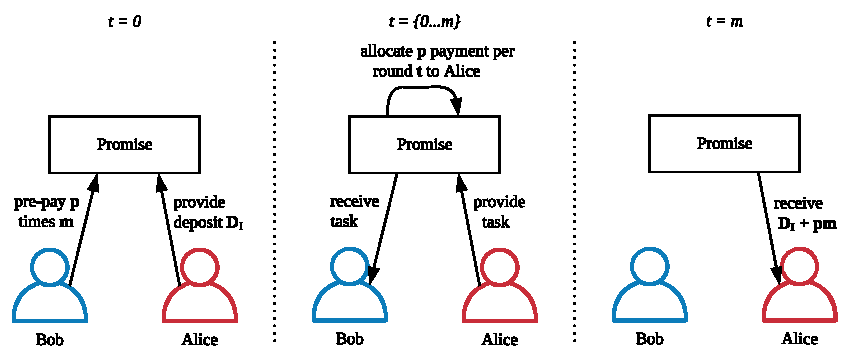
\includegraphics[width=\textwidth]{figures/protocol.pdf}
    \caption{\sys allows intermediaries (Alice) to lock less initial deposit $D_I$ and use payments $p_i$ provided by users (Bob) as additional deposit. The initial deposit and payments are locked for a period of time $m$ determined by Bob. Only when Alice behaves honestly for the entire period $m$ can Alice withdraw her initial deposit $D_I$ and the payments $pm$.}
    \label{fig:promise}
\end{figure}


\dom{Introduce the protocol}

\subsection{Protocol}

The \sys protocol consists of three steps.
We denote the intermediary as $A$, the user as $B$, and the smart contract implementing \sys as $P$.
We assume that $A$ and $B$ have agreed the total payment and the period over which the payment is to-be-paid in advance.

\begin{enumerate}
    \item At $t=0$. $B$ locks $pm$ payments in $P$.
    \item At $t=0$. $A$ locks the initial deposit $D_I$ in $P$.
    \item At $t=1$ until $t=m$. $A$ provides the agreed task to $B$. $P$ allocates one payment $p$ to $A$, if (i) $A$ provides a proof to $P$ that the task was completed, or (ii) $B$ does not provide a fraud proof that $A$ did not provide the task within a determined time~\cite{Al-Bassam2018}.
    \item At $t=m$. $A$ withdraws $pm$ and $D_I$ from $P$.
\end{enumerate}



To argue about the security of \sys, we introduce two concepts: (i) temporality and (ii) a likelihood of users exiting the system upon the counterparty cheating.

\subsection{Introducing Time}
We introduce temporality as follows.
Denoting time by $t$, we define the period for which Bob locks Alice's payments as $\tau$, such that if Bob makes a payment every period $t$ then $\tau=m$.
Let $m$ denote the number of payments that Bob makes into escrow.
Discounting is also introduced, where $0<\delta<1$ denotes the discount factor of an agent's valuation of future utility, i.e. the notion that the future is worth less than the present.
We argue that an agent can spent received payments somewhere else or potentially invest the payment for a profit.
Hence, the agent faces an opportunity cost for delayed payments.
% because it is in the future.
% \rk{"because it is in the future" I really find this too much of a simplification.}
The payoffs to Alice and Bob are as follows. 

\begin{equation}
\label{eq:time_alice}
\Pi_A(t) = 
\begin{cases}
    \sum_{t=0}^{m} \big( \frac{\delta}{1+r} \big)^{\tau} ( p - \mathrm{E}[r]D_{I}), & \text{if Alice is honest} \\
    % \big( \frac{\delta}{1+r} \big)^{m} pm - D_{I}((1+\mathrm{E}[r])^{m}-1), & \text{if Alice is honest} \\
    \sum_{t=0}^{m} \big( \frac{\delta}{1+r} \big)^{t} (V_A - \mathrm{E}[r]D_{I}-D_{I}), & \text{if Alice cheats} \\
\end{cases}
\end{equation}

% where 

% \begin{equation}
% \label{eq:status-quo_alice_cheat}

% \end{equation}

Bob receives the following payoff, depending on Alice's behavior.

\begin{equation}
\label{eq:time_bob}
\Pi_B (t) = 
\begin{cases}
\sum_{t=0}^{m} \big( \frac{\delta}{1+r} \big)^t (V_B - p - \mathrm{E}[r]p(m-t)) - c, & \text{if Alice is honest} \\
\sum_{t=0}^{m} \big( \frac{\delta}{1+r} \big)^t (D_{I} -V_B -c) , & \text{if Alice cheats} \\
\end{cases}
\end{equation}


\subsection{Termination Probability}
Lowering Alice's initial collateral to $D_I$ increases the risk of Alice cheating Bob.
% As shown in Eq. (\ref{eq:time_alice}), Alice will misbehave if her payoff for cheating is higher than her provided collateral $D_I$ plus the sum of payment $pm$.
Specifically, in the first round, Alice's collateral is the lowest since she has not provided the service yet and has not added any payment into her collateral pool.
% \dom{Note for a later point: Lemma: Given a single-shot game between Alice and Bob. If Alice decides to cheat on Bob at $t=0$, then Alice cheats in all subsequent rounds on Bob.}
% By reducing her collateral we essentially promote cheating.
% However, we argue that in practice Bob would leave the protocol after a certain number of times he is being mistreated, \emph{if he has another choice}.
% Therefore, we introduce an exit probability $\beta$ for Bob.

Eq. (\ref{eq:status-quo_alice}) and (\ref{eq:time_alice}) implicitly assume that Alice and Bob are playing a one-shot game ad infinitum.
% Under this framework, Bob would happily being tricked out of his $V_B$ again and again by Alice.
We argue that Bob exits a protocol after being cheated too often, encoded in the function $\beta \to [0,1)$ describing the likelihood that Bob remains in the protocol.
Each time Bob gets cheated, $n_c$, the lower the probability that Bob continues to participate.
Each user can have its own $\beta$ function where users might choose to never participate again in a protocol after being cheated once and others might tolerate a higher number of incidents.
This changes Alice's payoff for the protocol.
% Hence, if Alice considers $m$ rounds of the game, she receives the following payoffs:

\begin{equation}
\label{eq:promise_alice}
\Pi_A(t) = 
\begin{cases}
    \big( \frac{\delta}{1+r} \big)^{m} pm - D_{I}((1+\mathrm{E}[r])^{m}-1), & \text{if Alice is honest} \\
    \sum_{t=0}^{m} \big( \frac{\delta}{1+r} \big)^{t} \beta (V_A - \mathrm{E}[r]D_{I}-D_{I}), & \text{if Alice cheats} \\
\end{cases}
\end{equation}

% Bob's payoffs are as follows:
% \begin{equation}
% \label{eq:promise_bob}
% \Pi_B (t) = 
% \begin{cases}
% \sum_{t=0}^{m} \big( \frac{\delta}{1+r} \big)^t (V_B - p - \mathrm{E}[r]p(m-t)) - c, & \text{if Alice is honest} \\
% \sum_{t=0}^{m} \big( \frac{\delta}{1+r} \big)^t \beta (D -V_B -c) , & \text{if Alice cheats} \\
% \end{cases}
% \end{equation}


As $\beta$ decreases, the payoff to Alice converges to $0$ as $n \rightarrow \infty$.
For Alice, we increase the motivation to behave honestly by (i) providing a sum of payments $mp$ that Bob locks in the protocol, and (ii) the fear of Bob leaving the protocol altogether if she cheats. % as expressed by $\frac{\beta}{n_c}$.
As Bob chooses $m$ and $\tau$, he has a direct influence on Alice's expected payoff.
By setting large $m$ and $\tau$ and being able to quit the protocol upon cheating, he can essentially force rational Alice to behave honestly.
% for cheating converges to $0$, leaves Alice no other rational choice than to act honestly.
Overall, Alice can join protocols with less initial collateral while providing Bob with the option to use ongoing payments as an additional security measurement.
% For Alice, we can see that whether she behaves honestly or cheats, if $D_I+p=D$, her payoffs remain the same.
% However, the difference is that it is now easier for Alice to participate in the system and offer a service to Bob, since the deposit she has to provide, $D_I<D$. 
% For Bob, his utility is improved whether Alice is honest or cheats, since $c_L<C$.



%-------------------------------------------------
%---------------Security------------------------
%-------------------------------------------------

\section{Security Analysis}
\label{sec:security}

% We argue about the security of adding \sys to an existing protocol.
\sys aims to fulfill the following properties:

\begin{enumerate}
    \item \textbf{Security of funds}: Payments $p$ (future and current) provided by a user as well as deposits $D$ by intermediaries cannot be stolen. This property is fulfilled by implementing the escrow as a smart contract on a ledger with a functionality and appropriate security parameters as described in~\cite{garay2016bitcoin,gervais2016security}. 
    \item \textbf{Cost reduction for users}: Bob is able to reduce transaction costs $c$ by paying for multiple rounds $m$ of services for payment $p$ in advance.
    \item \textbf{Collateral reduction for intermediaries}: Alice is able to provide a lower deposit $D_I$ than the deposit required in a single-shot game setting $D$ while Bob enjoys the same level of security against Alice.
    \item \textbf{Sybil resistance}: It is not individually rational for Alice to increase her payoff $\Pi$ by cheating Bob in one round and provide the service honestly in the next rounds.
\end{enumerate}

% \subsection{Security of funds}
% Both Alice and Bob store their funds in escrow.
% The escrow needs to be securely implemented as a smart contract.
% % As such, funds are secure given that the underlying ledger functionality is secure.
% The \sys smart contract is required to monitor the status of the service provided by Alice to Bob, such that any potential safety or liveness failure in the target protocol is detected, and any locked payments held in escrow by the contract are released to Bob upon detection. If no failures are detected during the pre-agreed period, the smart-contract allows Alice to withdraw her earned payments.

% The security of operations performed in this smart contract is determined by the guarantees of the underlying ledger. Extensive discussion of this is outside the scope of this paper and we refer the reader to~\cite{garay2016bitcoin,gervais2016security}. We assume in our work that the safety or liveness provisions of the underlying ledger are not violated. %is operated by an honest majority such that no .

\subsection{Cost Reduction for Users}
Assume that Alice behaves honestly.
If a user pays every round $t$ for the service provided by Alice, then his payoff per round is $V_B - p - c$. % where $V_B$ is his private value for getting the service, $p$ the payment he makes and $c$ the cost for doing the payment.
However, locking multiple payments incurs opportunity cost.
This cost is lowered at every time step as the payments are assigned to the intermediary.
Hence, Bob starts with an opportunity cost of $\mathrm{E}[r]pm$ at $t=0$ and $\mathrm{E}[r]p(m-1)$ at $t=1$.
Generalizing this for $t$ rounds, leaves us with $\mathrm{E}[r]p(m-t)$. % at every time step $t$. % from today's perspective.
The user locks future payments when the sum of the transaction costs $c$ for $m$ payments is greater than the opportunity cost for locking additional payments plus the single transaction cost for making the prepayments.
Hence, the boundary for a user to choose \sys as individually rational choice maximizing his payoff is given by:

\begin{align}
\label{eq:decision-bound-user}
    \sum_{t=1}^m \big( \frac{\delta}{1+r} \big)^t c = \sum_{t=0}^m \big( \frac{\delta}{1+r} \big)^t \mathrm{E}[r]p(m-t)
\end{align}

% Provided the left hand side of Eq. (\ref{eq:decision-bound-user}) is greater, Bob should use \sys to lock multiple payments $pm$ as it is his individually rational choice that maximizes his payoff $\Pi_B$.

\subsection{Collateral Reduction and Sybil Resistance}

% Alice reduces her initial collateral with \sys.% from $D$ to $D_I$ where $D_I < D$.
% While this lowers her entry barrier, arguably this makes it easier for Alice to cheat in the protocol as she has less at stake.
% By introducing $\beta$ we Alice's desire to cheat is reduced.
% More formally, 
We can calculate the decision bound for Alice's individually rational choice to cheat Bob by comparing the two options in Eq. (\ref{eq:promise_alice}).
% \begin{equation}
%     \big( \frac{\delta}{1+r} \big)^{m} pm - D_{I}((1+\mathrm{E}[r])^{m}-1) =
%     \sum_{t=0}^{m} \big( \frac{\delta}{1+r} \big)^{t} \beta (V_A - \mathrm{E}[r]D_{I}-D_{I})
% \end{equation}
We can re-arrange this equation to determine $\beta$:
\begin{equation}
    \label{eq:beta}
    \beta = \frac{\big( \frac{\delta}{1+r} \big)^{m} pm - D_{I}((1+\mathrm{E}[r])^{m}-1)}{\sum_{t=0}^{m} \big( \frac{\delta}{1+r} \big)^{t} (V_A - \mathrm{E}[r]D_{I}-D_{I})}
\end{equation}
% \dom{re-arrange for $\beta$}

Similarly, Bob can determine how high $D_I$ should be under the assumption that he knows $V_A$ and the parameters $r$ and $\delta$.

% \dom{re-arrange for $D_I$}
\begin{equation}
    \label{eq:d_initial}
    D_I = \frac{\big( \frac{\delta}{1+r} \big)^{m} pm - \sum_{t=0}^{m} \big( \frac{\delta}{1+r} \big)^{t} \beta V_A}{ ((1+\mathrm{E}[r])^{m}-1) - \sum_{t=0}^{m} \big( \frac{\delta}{1+r} \big)^{t} \beta (\mathrm{E}[r]-1)}
\end{equation}

Assuming that $\beta$ is lowered aggressively, i.e.\ Bob tolerates only few task violations $n_c$, Alice  chooses to be honest as this maximizes her payoff.
Being honest with a reduced collateral $D_I$ is thereby the individually rational choice.
Given that Bob is aware for the involved parameters $V_A$, $r$, and can set the parameters $p$ and $m$ himself, Bob is able to calculate at which likelihood he should exit a given protocol given by Eq. (\ref{eq:beta}).
Similarly, Bob can decide which level of colalteral $D_I$ is sufficent for him using Eq.(\ref{eq:d_initial}).

% \subsection{Sybil resistance}
\subsubsection{Sybil Identities}
We argue that if $\beta$ is lowered aggressively, Alice can do no better than being honest.
However, if there is a non-negligible probability that Bob remains in the protocol after being cheated once, Alice can try to create a Sybil identity $A'$ to (i) cheat Bob in round $t=0$ and (ii) behave honestly in round $1$ to $m+1$.
Hence, Bob can only be sure to prevent Alice from executing a Sybil attack, if $\beta = 0$.

\subsection{Beta Factor Over Time}
The $\beta$ factor set by Bob is the crucial security parameter for Bob given we are in a permissionless system.
We argue that setting the $\beta$ factor depends on Bob's reliance on participating in a protocol.
If Bob \emph{requires} the service Alice provides and there is \emph{no alternative} to the protocol in which Alice operates, Bob is faced with a \emph{monopoly}.
In a monopoly Bob $\beta$ likely never approaches 0 as Bob is forced to tolerate Alice's misbehavior.
To protect Bob, \sys requires that $D_I$ of Alice is close or equal to $D$ in a monopoly.
% Otherwise, Alice can create Sybil attacks on Bob or just outright cheat every round as Bob would try to use the service over and over.

The opposite market situation is \emph{perfect competition}.
Bob can choose from a wide selection of service providers to interact with\footnote{
However, as we lack strong identities, these service providers could all be Sybil identities of Alice.
Recognizing that perfect competition exists is a challenging task and we leave this as future work.}.
Assuming perfect competition exists, Bob has the choice to leave a protocol any time.
As an example, we could imagine Bob choosing between using a payment hub like NOCUST or a payment channel network like Lighting to obtain scalable and cheap payments.
For simplicity of argument, we assume that Bob is indifferent if he pays in Bitcoin or Ether.
If Bob would be cheated on by an intermediary in NOCUST, he could switch to using the Lightning Network.
In turn, Bob can set $\beta$ to 0.
In these cases we can substantially lower the initial collateral $D_I$ using Eq. (\ref{eq:d_initial}).





%-------------------------------------------------
%---------------APPLICATION------------------------
%-------------------------------------------------


% \section{Applications}
% \label{sec:application}

% In this section we show how applying \sys to a set of popular protocols can improve them.
% % \aza{Shorten this to 1 paragraph and rather add 2 more applications! For the paper, it is better to even have a single paragraph, but highlight multiple protocols - rather than going into detail on 1 specific.}

% \subsection{NOCUST}

% NOCUST is a second-layer payment protocol whereby an untrusted intermediary operates a commit-chain to facilitate payments between its users~\cite{Khalil2019NOCUST}. We consider a scenario where Alice is the intermediary commit-chain operator, and Bob is a payment recipient. In this setting we propose to employ \sys as follows: Any fee to be paid by Bob to Alice in exchange for the delivery of an incoming payment would be locked as collateral that Bob could claim if the NOCUST protocol fails. Over time, the fees locked in \sys would grant Bob instant finality over larger payments, increasing the utility of the service.


% % We consider a scenario where Alice is the intermediary commit-chain operator, and Bob is a payment recipient. Alice can effectively deliver payments from other users to Bob without Alice having to put up additional collateral. However, without collateral, Bob has to wait for two rounds of the protocol to succeed before being guaranteed finality of an incoming payment. This delay in finality may be too long for certain use cases. 

% % Using NOCUST with additional collateral by Alice, however, can provide instant finality for Bob. In this case, Alice puts up an amount of collateral that is equal to what Bob expects to receive within two rounds of the protocol, such that if the protocol fails and pending payments are reverted, the collateral put up by Alice can act as a reimbursement for any expenses Bob may have incurred before finalization. For example, in a sale scenario, Bob could release some goods immediately after Alice promises to deliver the payment for them, instead of waiting two rounds for guaranteed finality. If Alice fails to deliver the payment, her collateral would paid to Bob to cover the cost of the goods.

% % In this setting we propose to employ \sys as follows: Any fee to be paid by Bob to Alice in exchange for the delivery of an incoming payment would be locked as collateral that Bob could claim if the NOCUST protocol fails. This gradually increases how reliable Bob perceives Alice to be as an intermediary as more fees are accumulated towards reimbursing Bob for any potential damages. If Bob wishes to utilize Alice's service with minimal risk, Bob would not release any goods in return for incoming payments until Bob is guaranteed finality. Over time, the fees locked in \sys would grant Bob instant finality over larger payments, increasing the utility of the service.

% \subsection{XCLAIM}

% XCLAIM is a protocol that allows users to transfer assets between heterogeneous decentralized ledgers using a collateralized intermediary~\cite{Zamyatin2019XCLAIM}.
% Instead of relying on a trusted third party like a centralized exchange, the intermediary must provide a collateral to ensure that she does not steal the coins she holds in custody.
% She has to verify correctness of her actions by submitting transaction inclusion proofs to the smart contracts that augments the protocol.
% \sys can be applied such that Alice locks some initial collateral $D_I$ and issues backed-tokens using this collateral.
% Bob, using her services, is able to lock the future payments of Alice to allow him to transfer more assets between the ledgers.

% \subsection{TrueBit}
% TrueBit is a protocol in which a set of intermediaries provide computation services~\cite{teutsch2017scalable}.


% \subsection{Dai stablecoin}

% Dai is a stablecoin in which intermediaries provide collateral to open so-called Collateralized Debt Positions (CDPs)~\cite{Maker2017Dai}.
% The collateral serves as a backing mechanism to ensure that the price of 1 Dai equals 1 USD.


% \subsection{SmartPool}
% \toaza{If you want to have this added, please add it.}

% \toaza{Please add XCLAIM}

% High level desc. of applications + how \sys can be applied.
% Suggestions:
% \begin{itemize}
%     \item XCLAIM
%     \item SmartPool
%     \item What else? PISA, MakerDAO, Stablecoins, ...
% \end{itemize}

%%%%%%%%%%%%%%

%-------------------------------------------------
%---------------Application------------------------
%-------------------------------------------------

\section{Application}
\label{sec:application}

\subsection{NOCUST}

NOCUST is a second-layer payment protocol whereby an untrusted intermediary operates a commit-chain to facilitate payments between its users~\cite{Khalil2019NOCUST}. We consider a scenario where Alice is the intermediary commit-chain operator, and Bob is a payment recipient. In this setting we propose to employ \sys as follows: Any fee to be paid by Bob to Alice in exchange for the delivery of an incoming payment would be locked as collateral that Bob could claim if the NOCUST protocol fails. Over time, the fees locked in \sys would grant Bob instant finality over larger payments, increasing the utility of the service.


We consider a scenario where Alice is the intermediary commit-chain operator, and Bob is a payment recipient. Alice can effectively deliver payments from other users to Bob without Alice having to put up additional collateral. However, without collateral, Bob has to wait for two rounds of the protocol to succeed before being guaranteed finality of an incoming payment. This delay in finality may be too long for certain use cases. 

Using NOCUST with additional collateral by Alice, however, can provide instant finality for Bob. In this case, Alice puts up an amount of collateral that is equal to what Bob expects to receive within two rounds of the protocol, such that if the protocol fails and pending payments are reverted, the collateral put up by Alice can act as a reimbursement for any expenses Bob may have incurred before finalization. For example, in a sale scenario, Bob could release some goods immediately after Alice promises to deliver the payment for them, instead of waiting two rounds for guaranteed finality. If Alice fails to deliver the payment, her collateral would paid to Bob to cover the cost of the goods.

In this setting we propose to employ \sys as follows: Any fee to be paid by Bob to Alice in exchange for the delivery of an incoming payment would be locked as collateral that Bob could claim if the NOCUST protocol fails. This gradually increases how reliable Bob perceives Alice to be as an intermediary as more fees are accumulated towards reimbursing Bob for any potential damages. If Bob wishes to utilize Alice's service with minimal risk, Bob would not release any goods in return for incoming payments until Bob is guaranteed finality. Over time, the fees locked in \sys would grant Bob instant finality over larger payments, increasing the utility of the service.

\subsection{Implementation}

We implement \sys in Solidity

%-------------------------------------------------
%---------------RELATED WORK------------------------
%-------------------------------------------------

\section{Related Work}
\label{sec:related}


% Relate to finance.

% \tolgu{Add related work from finance. The principle of pre-payment is not new, but only with smart contracts we can actually provide some guarantees that the funds will be returned to the users in if there is no misbehavior, i.e. cannot be stolen.}

There are two strands of related literature.
The first one comes from the financial world covering (advance) payments for financial contracts.
The second strand comes from the more recent work in decentralized ledgers.
In the economics literature, a wide range of work focuses on secured debt, such as ~\cite{scott1977bankruptcy,stulz1985analysis}.
However, these concepts rely on trust on third parties to maintain security in the debt and payment positions.
\sys replaces this third-party trust by holding advance payments in a smart contract escrow.
%which shows that some profitable projects will not be undertaken by a firm which can finance them only with equity or unsecured debt, but will be undertaken by a firm which can finance them with secured debt.
% \cite{boot1994moral} considers moral hazard and secured lending in the context of an infinitely repeated credit market game. 
% In addition, the issuance of secured debt has been argued to increase the value of a firm~\cite{scott1977bankruptcy}.
% Other work focuses on the efficiency secured debt under conditions of imperfect information~\cite{triantis1992secured}.
% Another branch of work relates to down payments (a payment made for something bought on credit)~\cite{engelhardt}. 
% ,mayer1996gifts,engelhardt1994house
%of secured debt~\cite{hill2001secured}, and 

On the second strand, Balance is a protocol that allows intermediaries to lower their collateral over time~\cite{Harz2019Balance}.
It operates at the other end of \sys: instead of lowering the initial collateral, the more an agent behaves honestly, the higher the reduction of collateral.
% Balance requires the highest collateral to be provided at the start of the interaction between agents and makes the assumption that payments are close to 0 (i.e.\ there is perfect competition).
\sys and Balance can be combined together to first reduce initial collateral when bootstrapping a new protocol and then lower collateral requirements for established agents over time.
Teutsch et al. discuss bootstrapping a token for verifiable computations~\cite{Teutsch2019Boostrap}.
% This work discusses how to enable users, like Bob, to obtain the required funds to participate in TrueBit.
Their proposal includes a governance game that allows to exchange special governance tokens into collateral tokens (for intermediaries) and utility tokens (for users).
Last, the idea of bundling payments together is also introduced in ~\cite{Berg2018} to create subscriptions for services of agents.
\sys extends this idea to allow collateral reduction for intermediaries.

% Other related work?
% \todom{Can you cover this? Does not have to be much, we have limited space.}
% \begin{itemize}
%     \item Balance
%     \item New paper by Teutsch
%     \item Payment streaming \url{https://github.com/ethereum/EIPs/issues/1620}
% \end{itemize}

%-------------------------------------------------
%---------------CONCLUSION------------------------
%-------------------------------------------------

\section{Conclusion}
\label{sec:conclusion}

We present \sys, a system that allows intermediaries to lower the initially locked collateral.
The core assumption for the security of \sys is that a user Bob is able to lock a number of payments up front and exit the protocol when Alice cheats.
This allows Alice to reduce her initial collateral requirement, allowing protocols that adopt \sys to lower the burden on intermediaries.
Bob is able to reduce his transaction cost as he transfers a sum of payments.
Further, Bob is able to receive the service in full --- for the entire period he pre-paid --- or he is refunded the entire sum of payments.
We have introduced a semi-formal model for \sys.
We discuss the security and the effect of the $\beta$ parameter, but leave formal proofs of the security properties as future work.


\bibliographystyle{splncs04}
\bibliography{bib/blockchain,bib/references}

\end{document}
